% This is text associated with the open textbook "Open Electromagnetics"
% See immediately below for author, date
% This work is licensed under the Creative Commons Attribution-ShareAlike 4.0 International License. (CC BY-SA 4.0) 
% To view a copy of the license, visit http://creativecommons.org/licenses/by-sa/4.0/

%ORB TITLE Reactance of the Electrically-Short Dipole
%ORB AUTHOR 0        # S.W. Ellingson, Virginia Tech (ellingson@vt.edu)
%ORB DATE 20191127   # yyyymmdd
%ORB ABSTRACT 

\label{m0210_Reactance_of_the_Electrically-Short_Dipole} % <-- Must match name of this file and module directory name.  Don't mess with this!
\index{antenna!electrically-short dipole (ESD)|(}

For any given time-varying voltage appearing across the terminals of an electrically-short antenna, there will be a time-varying current that flows in response.  The ratio of voltage to current is impedance.  Just as a resistor, capacitor, or inductor may be characterized in terms of an impedance, any antenna may be characterized in terms of this impedance.
The real-valued component of this impedance accounts for power which is radiated away from the antenna 
(Section~\ref{m0207_Total_Power_Radiated_by_an_Electrically-Short_Dipole}) and dissipated within the antenna 
(Section~\ref{m0208_Total_Power_Dissipated_by_an_Electrically-Short_Dipole}).
The imaginary component of this impedance -- i.e., the reactance -- typically represents energy storage within the antenna, in the same way that the reactance of a capacitor or inductor represents storage of electrical or magnetic energy, respectively. 
In this section, we determine the reactance of the electrically-short dipole (ESD).

{\bf Reactance of a zero-length dipole.}
We begin with what might seem initially to be an absurd notion: A dipole antenna having zero length.  
However, such a dipole is certainly electrically-short, and in fact serves as an extreme condition from which we can deduce some useful information.

Consider Figure~\ref{m0210_fTLonly}, which shows a zero-length dipole being driven by a source via a transmission line.
%
\begin{figure}[b!] % <--- "[b!]" for first figure in section *only*; delete for 2nd and subsequent figures
\begin{center}
\pdftooltip{{  % note double braces
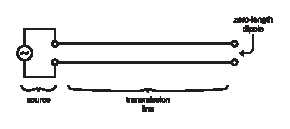
\includegraphics[width=3in]{modules/m0210_ZeroLengthDipole.eps} 
% https://commons.wikimedia.org/wiki/File:Zero-Length_Dipole_Open_Circuit.svg
}}{A source connected to a transmission line, ending in an open circuit labeled "zero-length dipole".}
\end{center}
\centerline{\scriptsize 
\copyright~\hyperref[m0210_fTLonly_Credit]{S.\ Lally} 
\href{https://creativecommons.org/licenses/by-sa/4.0/}{CC BY-SA 4.0} 
} % \centerline 
\caption{
\label{m0210_fTLonly}
Transmission line terminated into a zero-length dipole, which is equivalent to an open circuit.
}
\end{figure}
%
It is immediately apparent that such a dipole is equivalent to an open circuit.
So, the impedance of a zero-length dipole is equal to that of an open circuit.

What is the impedance of an open circuit?
One might be tempted to say ``infinite,'' since the current is zero independently of the voltage.
However, we must now be careful to properly recognize the real and imaginary components of this infinite number, and signs of these components.
In fact, the impedance of an open circuit is $0-j\infty$. 
One way to confirm this is via basic transmission line theory; i.e., the input impedance of transmission line stubs.
A more direct justification is as follows: 
The real part of the impedance is zero because there is no transfer of power into the termination.
The magnitude of the imaginary part of the impedance must be infinite because the current is zero.  
The sign of the imaginary component is negative because the reflected current experiences a sign change (required to make the total current zero), whereas the reflected voltage does not experience a sign change (and so is not canceled at the terminals). 
Thus, the impedance of an open circuit, and the zero-length dipole, is $0-j\infty$.

{\bf Reactance of a nearly-zero-length dipole.}
Let us now consider what happens as the length of the dipole increases from zero.
Since such a dipole is short compared to a wavelength, the variation with length must be very simple.
The reactance remains large and negative, but can only increase (become less negative) monotonically with increasing electrical length. 
This trend continues until the dipole is no longer electrically short.
Thus, we conclude that the reactance of an ESD is always large and negative.
%
%%%%%%%%%%%%%%%%%%%%%%%%%%%%%%%%%%%%%%%%%%%%%%%
%ORB HIGHLIGHT
\begin{mdframed}[backgroundcolor=yellow!20,nobreak=true] 
The reactance of an ESD is very large and negative, approaching the reactance of an open circuit termination as length decreases to zero. 
\end{mdframed}
%%%%%%%%%%%%%%%%%%%%%%%%%%%%%%%%%%%%%%%%%%%%%%%

Note that this behavior is similar to that of a capacitor, whose impedance is also negative and increases toward zero with increasing frequency.
Thus, the reactance of an ESD is sometimes represented in circuit diagrams as a capacitor. 
However, the specific dependence of reactance on frequency is different from that of a capacitor (as we shall see in a moment), so this model is generally valid only for analysis at one frequency at time.

{\bf An approximate expression for the reactance of an ESD.}
Sometimes it is useful to be able to estimate the reactance $X_A$ of an ESD.  
Although a derivation is beyond the scope of this text, a suitable expression is (see, e.g., Johnson (1993) in ``Additional References'' at the end of this section):
%
\begin{equation}
X_A \approx -\frac{120~\Omega}{\pi L/\lambda} \left[ \ln{\left(\frac{L}{2a}\right)}-1 \right]
\label{m0210_eXA}
\end{equation}
%
where $L$ is length and $a\ll L$ is the radius of the wire comprising the ESD.
Note that this expression yields the expected behavior; i.e., $X_A\rightarrow-\infty$ as $L \rightarrow 0$, and increases monotonically as $L$ increases from zero.

%%%%%%%%%%%%%%%%%%%%%%%%%%%%%%%%%%%%%%%%%%%%%%%
%ORB EXAMPLE
~\\ \begin{example} 
\begin{mdframed}[backgroundcolor=brown!20,linecolor=brown!20]\raggedright
Reactance of an ESD. 
\\~\\
A dipole is 10~cm in length, 1~mm in radius, and is surrounded by free space.
What is the reactance of this antenna at 30~MHz?

{\bf Solution.}
The wavelength $\lambda=c/f \cong 10$~m, so $L = 10~\mbox{cm} \cong 0.01\lambda$.
This certainly qualifies as electrically-short, so we may use Equation~\ref{m0210_eXA}.
Given $a=1$~mm, we find the reactance $X_A \approx \underline{-11.1~\mbox{k}\Omega}$.
For what it's worth, this antenna exhibits approximately the same reactance as a 0.47~pF capacitor at the same frequency.

\end{mdframed}
% note figures will need to go between "\end{mdframed}" and "\end{example}"
\end{example}
%%%%%%%%%%%%%%%%%%%%%%%%%%%%%%%%%%%%%%%%%%%%%%%

The reactance of the ESD is typically orders of magnitude larger than the real part of the impedance of the ESD.
The reactance of the ESD is also typically very large compared to the characteristic impedance of typical transmission lines (usually 10s to 100s of ohms). 
This makes ESDs quite difficult to use in practical transmit applications.

%%%%%%%%%%%%%%%%%%%%%

{\bf Additional Reading:}
\begin{itemize}
\item R.C.\ Johnson (Ed.), \emph{Antenna Systems Handbook} (Ch.\ 4), McGraw-Hill, 1993.
\end{itemize}

%%%%%%%%%%%%%%%%%%%%%%

\index{antenna!electrically-short dipole (ESD)|)}

